%%%%%%%%%%%%%%%%%%%%% chapter.tex %%%%%%%%%%%%%%%%%%%%%%%%%%%%%%%%%
%
% sample chapter
%
% Use this file as a template for your own input.
%
%%%%%%%%%%%%%%%%%%%%%%%% Springer-Verlag %%%%%%%%%%%%%%%%%%%%%%%%%%
%\motto{Use the template \emph{chapter.tex} to style the various elements of your chapter content.}
\chapter{Open Questions and Potential Research Directions}
\label{open-research} % Always give a unique label
% use \chaptermark{}
% to alter or adjust the chapter heading in the running head

\abstract*{Since \mbox{U-LTE} is a nascent LTE technology, the coexistence of this technology and \mbox{Wi-Fi} remains one of the most active research topics and working areas. Based on observations obtained from the survey and our study presented in Chapters \ref{survey} and \ref{intro-NALT}, this chapter attempts to highlight a number of open research questions and issues. Potential solutions to those issues are also identified. Primarily, the cooperation of LTE and \mbox{Wi-Fi} so that they could have a better understanding of each other when operating in the same area using the same radio frequency band is suggested. Such understanding can be used to take more vigilant action and help to avoid aggressive channel access that could corrupt on-going transmissions and to design relevant protocols for a fair spectrum sharing.}

Since \mbox{U-LTE} is a nascent LTE technology, the coexistence of this technology and \mbox{Wi-Fi} remains one of the most active research topics and working areas. Based on observations obtained from the survey and our study presented in Chapters \ref{survey} and \ref{intro-NALT}, this chapter attempts to highlight a number of open research questions and issues. Potential solutions to those issues are also identified. Primarily, the cooperation of LTE and \mbox{Wi-Fi} so that they could have a better understanding of each other when operating in the same area using the same radio frequency band is suggested. Such understanding can be used to take more vigilant action and help to avoid aggressive channel access that could corrupt on-going transmissions and to design relevant protocols for a fair spectrum sharing.

\section{LTE-U-aware CSMA-CA and LTE-U with LBT}
\label{subsection:LTE-U-aware}

\mbox{LTE-U} mostly assumes neither coordination nor synchronization between itself and \mbox{Wi-Fi} system. \mbox{LTE-U}'s ``on'' and ``off'' cycles are only known by LTE devices themselves. Vice versa, \mbox{Wi-Fi} control and management frames are known by \mbox{Wi-Fi} devices themselves. This independent operation results in various transmission issues. First, in cases when \mbox{LTE-U}'s ``on'' duration is not sufficiently long while \mbox{Wi-Fi} exponential back-off procedure generates long back-off intervals, \mbox{Wi-Fi} STAs may not have a chance to utilize the channel when \mbox{LTE-U} is not active. Such a conservative channel access principle wastes the radio resources and results in \mbox{Wi-Fi}'s poor performance. Second, an unfinished \mbox{Wi-Fi} frame transmission that was started during the \mbox{LTE-U}'s ``off'' duration might be corrupted by the LTE frames once LTE switches to ``on'' cycle. Fig. \ref{figs:LTE-U-enhancement1} visualizes two examples.
\begin{figure}[!ht]
	\centering
	\includegraphics[width=1.0\columnwidth]{figs/LTE-U-enhancement1}
	\caption{Negative interactions between \mbox{LTE-U} and \mbox{Wi-Fi} systems.}
	\label{figs:LTE-U-enhancement1}
\end{figure}

To mitigate these issues, inter-RAT communications between LTE and \mbox{Wi-Fi} could be employed to inform \mbox{Wi-Fi} system the \mbox{LTE-U}'s ``on'' and ``off'' cycles. \mbox{Wi-Fi} system then can adapt its MAC protocol (i) to occupy the channel more opportunistically during \mbox{LTE-U}'s ``off'' period (but not to increase the collision probability among \mbox{Wi-Fi} STAs) and (ii) to schedule frame transmissions in such a way that they will not step on the next \mbox{LTE-U}'s ``on'' cycle. Further, frame collisions could be mitigated by incorporating some form of LBT/CCA into \mbox{LTE-U}. Specifically, CCA should be performed before activating \mbox{LTE-U}'s ``on'' cycle. If the channel is detected busy, \mbox{LTE-U}'s ``on'' cycle is deferred.

\section{LAA-LTE with Exponential Back-off}
\label{subsection:exp-back-off}

While LBT, as a general approach, can be a good basis for coexistence of \mbox{LAA-LTE} and \mbox{Wi-Fi}, the LBE LBT in its current form (as introduced by European regulations) which is adopted for \mbox{LAA-LTE} is still unfair to \mbox{Wi-Fi}. \mbox{LAA-LTE} nodes impact \mbox{Wi-Fi} nodes in terms collision rate and probability of successful channel access more than similar \mbox{Wi-Fi} nodes on the same carrier. This is not compliant with the objectives as listed in 3GPP LAA LTE Study Item \cite{LAA-LTE-SI}: ``LAA should not impact \mbox{Wi-Fi} services (data, video and voice services) more than an additional \mbox{Wi-Fi} network on the same carrier; these metrics could include throughput, latency, jitter, etc.''. One major contributing factor is, that while \mbox{Wi-Fi} applies exponential back-off rule, \mbox{LAA-LTE} simply applies fixed-size back-off rule. In order to illustrate this observation, consider the following: It is assumed that $W^{{\mbox{LAA}}}=31$, $W^{\mbox{Wi-Fi}}_{\min}=31$, and $W^{{\mbox{Wi-Fi}}}_{\max}=1023$. Then, as described in Section \ref{laa-lte}, \mbox{LTE-U} always backs off with contention window $W^{\mathrm{\mbox{LAA}}}=31$. For \mbox{Wi-Fi}, as described in Section \ref{collision-avoidance}, it backs off with contention window $W(0)=31$ for the initial transmission attempt. However, if collisions occur, it progressively doubles its contention windows to reduce the probability of a subsequent collision: $W(1)=63$ (the first re-transmission attempt), $W(2)=127$ (the second re-transmission attempt), $W(3)=255$ (the third re-transmission attempt), $W(4)=511$, $W(5)=1023$, $W(6)=1023$, and so on. Fig. \ref{figs:LAA-LTE-enhacement-back-off} compares how the contention windows of \mbox{LAA-LTE} and \mbox{Wi-Fi} changes in response to collisions.
\begin{figure}[!ht]
	\centering
	\includegraphics[width=1.0\columnwidth]{figs/LAA-LTE-enhacement-back-off}
	\caption{\mbox{Wi-Fi} exponential back-off competes for the channel more conservatively, compared to \mbox{LAA-LTE}.}
	\label{figs:LAA-LTE-enhacement-back-off}
\end{figure}

At present, there is no existing work that studies how an exponential back-off can help to improve the fairness between \mbox{LAA-LTE} and \mbox{Wi-Fi}. It is important to note that, compared to \mbox{Wi-Fi}, designing an exponential back-off protocol for \mbox{LAA-LTE} that employs OFDMA-based MAC layer might not be straightforward. In details, \mbox{Wi-Fi} adopts OFDM in the PHY layer and allows only one user to occupy the whole channel at one time. Its contention window is scaled respectively to the outcome (success or failure) of a frame transmission to given user. For LTE, OFDMA divides the system bandwidth into a series of Physical Resource Blocks (PRBs). Each PRB is composed of $12$ OFDM subcarriers. Different PRBs can be allocated to different users in a given subframe and multiple users can occupy the channel at the same time. This implies that the rule governing the adaptation of contention window of \mbox{LAA-LTE} is required to be more sophisticated than that of \mbox{Wi-Fi}. In addition to back-off procedure design, there are two other interesting questions: (i) how exponential back-off could (negatively) affect the performance and efficiency of \mbox{LAA-LTE}; and (ii) what could be appropriate values for \mbox{LAA-LTE}'s operation parameters.

A side note is that, according to \cite{U-LTE-FCC-Cisco-2015}, 3GPP is now having a working agreement to use a LBT mechanism with exponential back-off. At this moment, \mbox{LAA-LTE} standard is not yet finalized by 3GPP and no information is publicly available. ETSI is also devising a set of minimum ``fairness'' requirements as part of EN 301 893 standard for ``5 GHz high performance wireless access systems'' in Europe (scheduled to be completed by the end of 2015).

\section{Wi-Fi-aware LTE-U and LAA-LTE}
\label{subsection:Wi-Fi-aware}

As addressed in Section \ref{collision-avoidance}, RTS/CTS and NAV are effective and important mechanisms employed by the IEEE 802.11 CSMA-CA protocol to reserve the channel and avoid collisions. However, since \mbox{U-LTE} and \mbox{Wi-Fi} are not collaborating, \mbox{Wi-Fi}'s NAV information carried by RTS, CTS, and data frames is not known by \mbox{U-LTE} devices. In other words, while \mbox{Wi-Fi} STAs defer their transmissions until ongoing frame exchanges are done, \mbox{U-LTE} devices do not respect \mbox{Wi-Fi} reservation and may start their transmissions at any time, as shown in Fig. \ref{figs:LTE-U-enhancement-RTS-CTS-NAV}.
\begin{figure}[!ht]
	\centering
	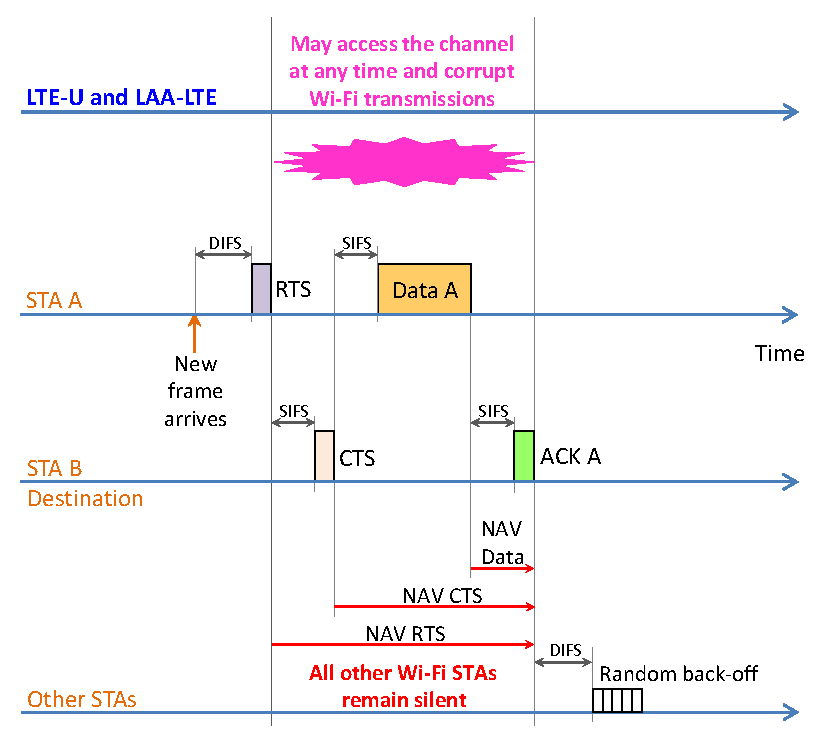
\includegraphics[width=0.7\columnwidth]{figs/LTE-U-enhancement-RTS-CTS-NAV}
	\caption{\mbox{U-LTE} may cause channel collisions with \mbox{Wi-Fi} at any time.}
	\label{figs:LTE-U-enhancement-RTS-CTS-NAV}
\end{figure}
This may result in a high rate of channel collisions and corrupt both \mbox{Wi-Fi} and \mbox{U-LTE} transmissions. As visualized Fig. \ref{figs:LTE-U-enhancement-RTS-CTS-NAV}, an \mbox{U-LTE} transmission could accidentally destroy the whole \mbox{Wi-Fi} transmission session composing of RTS, CTS, data, and ACK frames (at the same time, \mbox{U-LTE} frame is also corrupted by \mbox{Wi-Fi} frames). Mechanisms that provide \mbox{U-LTE} with information on \mbox{Wi-Fi} activities to avoid such transmission corruptions could be therefore very beneficial.

\section{Collaborative U-LTE and Wi-Fi}
As mentioned so far, almost all existing works dealing with \mbox{U-LTE} and \mbox{Wi-Fi} coexistence assume non-cooperative approach which does not required any information exchange between these two networks. LTE is simply additionally equipped with some mechanisms to friendly share the same channel with existing \mbox{Wi-Fi} networks. The authors in \cite{U-LTE-5G-2015, Coordinated-LTE-U-Wi-Fi-2015} carry out preliminary investigations towards this direction. However, only conceptual network architectures and mechanisms and are presented. Collaborative approaches is quite interesting since it may result in better coexistence by sharing information between different radio access technologies (RATs) and enabling global/local optimizations. Some benefits of such approaches has been outlined in subsections \ref{subsection:LTE-U-aware} and \ref{subsection:Wi-Fi-aware}. This approach, on the other hand, may be challenging since it needs additional network infrastructure/entities and set of protocols for inter-RAT communications. They are required for discovery of neighboring radio systems, selecting operating channels/transmission power, etc., for radio systems, and providing some level of fair and/or efficient use of available channels. 

\section{Inter-operator U-LTE Coexistence}
In addition to coexistence between \mbox{U-LTE} and \mbox{Wi-Fi}, coexistence among \mbox{U-LTE} systems deployed by different operators running in a shared band is also a critical concern. This concern is more pronounced in high density urban areas with a very large number of devices/system running different protocols. Work in \cite{LTE-U-ICC-WS-2015} presents a preliminary study on this and the results show that LBT mechanisms can increase the network throughput since collisions can be mitigated. Work in \cite{Enhanced-LTE-U-thesis-2015} investigates the interactions between different LBT mechanisms when they are deployed in proximity of each other. Inter-operator \mbox{U-LTE} coexistence is especially important when multiple operators employ similar MAC protocols based on fixed contention windows that could be accidentally synchronized in channel access attempts and result in consecutive collisions. As a result, exponential back-off rules, inter-RAT communications, and collaborative interference management protocols could be promising approaches.

\section{Other Considerations on Coexistence}
Operations, system performance, and coexistence of radio networks highly depend on deployment scenarios. This is the main reason why a number of existing work supports \mbox{U-LTE} technology while the others call for further investigations and developments before deploying this technology. Also, different coexistence mechanisms are recommended for different scenarios. For a complete understanding of \mbox{U-LTE} impacts on \mbox{Wi-Fi}, a wide range of node and load densities should be considered. Additionally, performance of voice and video-related applications should be evaluated. For most of existing work, only throughput and channel access probability of \mbox{Wi-Fi} networks are evaluated. However, an insight to latency and jitter performance could be desirable and it would be interesting to take into account the operations and performance of recent \mbox{Wi-Fi} variants when coexisting with \mbox{U-LTE}.

\section{Emerging Wi-Fi Technologies and U-LTE}
With the current trends of future RANs, including network densification, heterogeneous networks (HetNet), Internet of Things (IoT), and the explosion of various applications (smart homes/cities, smart transportations, autonomous vehicles, etc.), numerous technological evolutions have been emerging. For time-sensitive applications (e.g., sensor and control for critical infrastructures and autonomous vehicles), data communications is required to be extremely reliable, robust, energy-efficient while being able to guarantee latencies in millisecond or sub-millisecond scale. These requirements urge for the developments of collaborative, well-controlled, and synchronous \mbox{Wi-Fi} MAC protocols (instead of distributed, random-access-based, and asynchronous IEEE 802.11 CSMA/CA that have been widely deployed). To this end, PCF and HCCA operation schemes (specified in IEEE 802.11/802.11e standards but not widely used) should be re-visited.

Despite the fact that PCF and HCCA allocate the channel to STAs in a well-controlled manner, their performance (in terms of throughput, latency, and power consumption) is still questionable due to their complexities and signaling overhead, especially in highly dense networks with a vast number of battery-operated devices exchanging short and bursty messages. Furthermore, it is compelling to understand their interaction and coexistence with \mbox{U-LTE}. While CFP and CAP are desired for time-sensitive applications, the aggressive operation of \mbox{U-LTE} in the same frequency band may render them impossible. Finally, protocols and enabling technologies for collaborations and synchronizations between PCF-/HCCA-based \mbox{Wi-Fi} and \mbox{U-LTE} appear to be essential and thus could be very interesting working areas.

%%%%%%%%%%%%%%%%%%%%%%%% referenc.tex %%%%%%%%%%%%%%%%%%%%%%%%%%%%%%
% sample references
% %
% Use this file as a template for your own input.
%
%%%%%%%%%%%%%%%%%%%%%%%% Springer-Verlag %%%%%%%%%%%%%%%%%%%%%%%%%%
%

\begin{thebibliography}{99.}%
\bibitem{LAA-LTE-SI}``{3GPP™} work item: Study on licensed-assisted access using {LTE} to unlicensed spectrum,'' 3rd Generation Partnership Project (3GPP).

\bibitem{U-LTE-FCC-Cisco-2015}M.~L. Brown, ``Current trends in {LTE-U} and {LAA} technology,'' Comments of Qualcomm Incoporated, Qualcomm Inc., Jun. 2015.

\bibitem{U-LTE-5G-2015}
A.~Al-Dulaimi, S.~Al-Rubaye, Q.~Ni, and E.~Sousa, ``{5G} communications race: Pursuit of more capacity triggers {LTE} in unlicensed band,'' \emph{IEEE Vehicular Technology Magazine}, vol.~10, no.~1, pp. 43--51, March 2015.

\bibitem{Coordinated-LTE-U-Wi-Fi-2015} S.~Sagari, S.~Baysting, D.~Saha, I.~Seskar, W.~Trappe, and D.~Raychaudhuri,``Coordinated dynamic spectrum management of {LTE-U} and {Wi-Fi} networks,''
in \emph{2015 IEEE International Symposium on Dynamic Spectrum Access Networks (DySPAN)}, Sept 2015, pp. 209--220.

\bibitem{LTE-U-ICC-WS-2015}A.~Voicu, L.~Simic, and M.~Petrova, ``Coexistence of pico- and femto-cellular {LTE}-unlicensed with legacy indoor {Wi-Fi} deployments,'' in \emph{2015 IEEE	International Conference on Communication Workshop (ICCW)}, June 2015, pp.2294--2300.

\bibitem{Enhanced-LTE-U-thesis-2015}A.~Kanyeshuli, ``{LTE} in unlicensed band: Medium access and performance evaluation,'' Master's thesis, University of Agder, Norway, May 2015.
\end{thebibliography}
